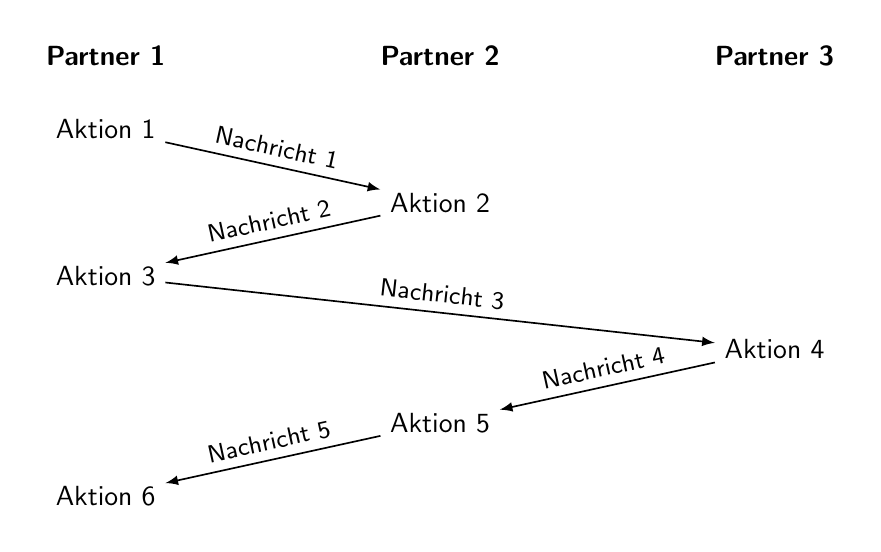
\begin{tikzpicture}[
every node/.append style={font={\sffamily}},
caption/.append style={font={\sffamily\bfseries}},
comm/.style={-latex,semithick},
msg/.style={midway,sloped,above,font={\sffamily\small}},
]
\matrix[row sep=3ex,column sep=25mm] {
\node[caption] {Partner 1};  & \node[caption] {Partner 2}; & \node[caption] {Partner 3}; \\
\node (A1) {Aktion 1}; & & \\
& \node (A2) {Aktion 2}; & \\
\node (A3) {Aktion 3}; & & \\
& & \node (A4) {Aktion 4};\\
& \node (A5) {Aktion 5}; & \\
\node (A6) {Aktion 6}; & & \\
};

\draw[comm] (A1)--(A2) node[msg] {Nachricht 1};
\draw[comm] (A2)--(A3) node[msg] {Nachricht 2};
\draw[comm] (A3)--(A4) node[msg] {Nachricht 3};
\draw[comm] (A4)--(A5) node[msg] {Nachricht 4};
\draw[comm] (A5)--(A6) node[msg] {Nachricht 5};

\end{tikzpicture}